\documentclass[12pt,letterpaper]{article}

% Compilador recomendado: pdfLaTeX
\usepackage[utf8]{inputenc}
\usepackage[T1]{fontenc}
\usepackage[spanish,es-tabla]{babel}
\usepackage{lmodern}
\usepackage[margin=2.5cm]{geometry}
\usepackage{amsmath,amssymb}
\usepackage{booktabs}
\usepackage{tabularx}
\usepackage{array}
\usepackage{graphicx}
\usepackage{subcaption}
\usepackage{float}
\usepackage{enumitem}
\usepackage{microtype}
\usepackage[hidelinks]{hyperref}

\graphicspath{{fotos/}}

\setlength{\parindent}{0pt}
\setlength{\parskip}{0.6em}
\renewcommand{\arraystretch}{1.2}
\setlist[itemize]{nosep}
\setlist[enumerate]{nosep}
\newcolumntype{Y}{>{\raggedright\arraybackslash}X}

\newcommand{\titulo}{
Maquinas de estados finitos
}

\begin{document}

\begin{titlepage}
    \centering

    {\large Instituto Tecnológico de Costa Rica\par}
    {\large Escuela de Ingeniería en Computadores\par}

    \vspace{1.5cm}

    {\large CE1107 --- Fundamentos de Arquitectura
    de Computadores\par}

    \vspace{1cm}

    {\Large\bfseries Proyecto Grupal 1\par}
    \vspace{0.5cm}
    {\LARGE\bfseries \titulo\par}

    \vspace{1cm}
    {\Large Propuesta de investigación\par}

    \vfill

    \textbf{Integrantes}\\
    Byron Josué Bolaños Porras, b.bolanos.1@estudiantec.cr \\
    Jose Andrés Chavarría Gamboa, j.chavarria.6@estudiantec.cr\\
    Isaac Arias Picado,  I.arias.2@estudiantec.cr \\
    Isac Marín Sirias, isacms@estudiantec.cr

    \vspace{1cm}

    \textbf{Profesor}\\
    Luis Chavarría Zamora

    \vspace{1cm}
    noviembre, 2026
\end{titlepage}

\section*{Resumen}

Se investiga el diseño de un sistema de control de acceso
para una puerta inteligente, implementado mediante una FPGA.
El sistema recibe símbolos procedentes de un detector de
dedos, forma contraseñas de tres dígitos y las compara con
las almacenadas en memoria. Una contraseña válida permite
alternar entre apertura y cierre, mientras una unidad
aritmético-lógica determina el ciclo de trabajo utilizado
para controlar el motor.

La propuesta organiza la solución en cuatro bloques:
adquisición de entradas, procesamiento de datos, control
secuencial y generación de salidas. La metodología combina
análisis de requisitos, diseño estructural, simulación
modular e integrada, síntesis en la FPGA y pruebas con
sensores, buzzer y motor reales. Las mediciones confirman
que el PWM reparte las velocidades de forma lineal y que
el temporizador cumple los tiempos programados. En una
maqueta de puerta corrediza el sistema abre y cierra en
las siete velocidades, después de bajar la frecuencia del
PWM a 10 Hz y de agregar contactos de final de carrera
que detienen el motor al llegar a cada tope.

\tableofcontents
\newpage

% ============================================================
% 1. PROBLEMA
% ============================================================

\section{Identificación del problema complejo de ingeniería
a investigar}

\subsection{Descripción del problema}

El proyecto plantea construir una puerta que permita el
acceso únicamente mediante contraseñas registradas. La
contraseña se introduce con una mano, utilizando seis
símbolos asociados a cantidades de dedos entre cero y cinco.
Cada intento contiene tres símbolos y no debe requerir
botones para confirmar individualmente sus dígitos
\cite{enunciado}.

La dificultad consiste en coordinar entradas físicas,
memoria, operaciones aritméticas, decisiones secuenciales
y actuadores. Una lectura inestable podría alterar una
contraseña; una transición incorrecta podría activar el
motor en un momento indebido; y una representación visual
inconsistente podría comunicar al usuario un estado
distinto del que mantiene el controlador.

Además, el diseño debe recordar si la puerta está abierta
o cerrada, permitir registrar y eliminar contraseñas,
incorporar un método de prueba y generar avisos sonoros.
La velocidad se obtiene mediante una ALU que interpreta
el primer dígito como operación y los dos restantes como
operandos.

\subsection{Pregunta de investigación}

¿Cómo diseñar y verificar un controlador estructural en
FPGA que coordine la captura de contraseñas, su validación
y el movimiento de una puerta, manteniendo coherencia
entre el estado lógico, las señales de actuación y la
información presentada al usuario?

\subsection{Factores que hacen complejo el problema}

\begin{itemize}
    \item Las entradas de sensores y botones no están
    necesariamente sincronizadas con el reloj de la FPGA.
    \item El sistema debe distinguir un intento completo
    de una ventana parcialmente capturada.
    \item La misma contraseña registrada debe permitir
    abrir o cerrar según la posición recordada.
    \item Las decisiones de autenticación, administración
    y prueba pueden competir por los mismos recursos.
    \item El control digital debe conectarse con una etapa
    de potencia y un mecanismo cuyo comportamiento depende
    de carga, fricción y alimentación.
    \item El enunciado exige una implementación estructural
    mediante ecuaciones booleanas y registros, sin
    \texttt{if}, \texttt{case} ni operadores ternarios en
    el circuito sintetizable.
\end{itemize}

\subsection{Alcance y restricciones}

El alcance comprende la lógica digital de los bloques de
entrada, datos, control y salidas, además de su conexión
en un módulo superior. La plataforma seleccionada en la
propuesta del equipo es una DE10-Standard con reloj de
50 MHz \cite{propuesta}.

El motor requiere una etapa externa de manejo y desacople;
no se alimenta directamente desde los pines de la FPGA.
La validación eléctrica y mecánica debe realizarse
separadamente de la simulación lógica.

El enunciado menciona siete velocidades y también un
resultado de tres bits entre cero y siete. La
implementación estudiada interpreta este resultado como
ocho niveles de ciclo de trabajo, incluidos apagado y
activación completa. Esta interpretación debe confirmarse
con el profesor.

% ============================================================
% 2. PROPUESTA
% ============================================================

\section{Diseño de una propuesta de investigación}

\subsection{Objetivo general}

Diseñar y evaluar un sistema modular de control de acceso
en FPGA, basado en lógica estructural y máquinas de
estados, que administre contraseñas y coordine el
movimiento de una puerta con información visual y sonora.

\subsection{Objetivos específicos}

\begin{enumerate}
    \item Definir interfaces coherentes entre los módulos
    de captura, memoria, cálculo, control y actuación.
    \item Implementar la identificación de intentos de
    tres símbolos y su comparación con dos espacios
    de contraseñas.
    \item Calcular una velocidad de tres bits mediante
    suma, resta, multiplicación y rotaciones.
    \item Generar PWM, dirección de motor, patrones
    sonoros y caracteres de siete segmentos.
    \item Verificar los módulos mediante referencias
    independientes y analizar sus límites antes de
    la evaluación física.
\end{enumerate}

\subsection{Hipótesis de trabajo}

La separación del sistema en módulos con interfaces
explícitas permitirá verificar sus funciones individuales
y detectar incompatibilidades antes de las pruebas
integrales. Si las decisiones secuenciales se expresan
mediante tablas y ecuaciones con prioridades definidas,
será posible coordinar el acceso y el movimiento sin
introducir ambigüedades funcionales entre bloques.

Esta hipótesis requiere tanto pruebas unitarias como
pruebas de integración. La aprobación de un módulo por
separado no demuestra por sí sola el funcionamiento
completo de la puerta.

\subsection{Arquitectura propuesta}

\begin{table}[H]
\centering
\small
\begin{tabularx}{\textwidth}{@{}p{2cm}YY@{}}
\toprule
Bloque & Responsabilidad & Componentes principales\\
\midrule
A: entradas &
Sincronizar, filtrar y capturar símbolos. &
Generador de habilitaciones, filtro de entradas y
ventana de captura.\\
B: datos &
Guardar contraseñas, comparar intentos y calcular
la velocidad. &
Memoria de dos espacios, comparador y ALU.\\
C: control &
Evaluar intentos y coordinar administración,
movimiento y prueba. &
Control de intentos, temporizador y FSM principal.\\
D: salidas &
Convertir órdenes en señales físicas y
representaciones visuales. &
PWM, control de motor, buzzer y displays.\\
\bottomrule
\end{tabularx}
\caption{Distribución funcional de la solución.}
\end{table}

El módulo superior conecta los cuatro bloques. La ventana
de captura alimenta el cálculo y la comparación; la FSM
almacena la velocidad aceptada y genera las órdenes de
escritura, borrado, temporización y actuación.

\subsection{Captura y administración de contraseñas}

El diseño utiliza una captura cada dos segundos. La
entrada de cinco bits se interpreta como un código de
cero o un único bit activo, que se convierte en un símbolo
entre cero y cinco. En el montaje cada dedo cubre una
fotorresistencia distinta y activa un solo bit, por lo
que la representación coincide con la salida del detector.

El control de intentos comienza al recibir un símbolo
distinto de cero y genera una indicación de intento
completo después de tres capturas válidas. Los símbolos
segundo y tercero sí pueden ser cero.

La restricción del primer símbolo es una decisión del
equipo asociada a las operaciones de la ALU, numeradas
del uno al cinco. Su aceptación debe verificarse respecto
al enunciado.

En administración se selecciona uno de dos espacios.
Si el intento coincide con una contraseña existente,
se elimina la coincidencia; si no coincide, se almacena
en el espacio seleccionado.

\subsection{Cálculo y control de velocidad}

La ALU entrega un resultado de tres bits, con
comportamiento circular:

\begin{equation}
s = R \bmod 8,
\qquad s \in \{0,1,\ldots,7\},
\end{equation}

donde $R$ corresponde al resultado de la operación
seleccionada. Las rotaciones se realizan sobre tres bits,
con una cantidad de giros equivalente a $B \bmod 3$.

El PWM tiene una frecuencia de 10 Hz. Con un reloj
de 50 MHz, el período contiene:

\begin{equation}
N=\frac{50\,000\,000}{10}=5\,000\,000
\text{ ciclos}.
\end{equation}

El número de ciclos activos se calcula como:

\begin{equation}
H(s)=\operatorname{round}\left(\frac{Ns}{7}\right),
\qquad
D(s)=\frac{H(s)}{N}.
\end{equation}

La propuesta inicial usaba 1 kHz. Durante las pruebas
físicas la frecuencia se redujo a 200 Hz y luego a
100 Hz, porque con pulsos tan cortos el motor no
arrancaba en las velocidades bajas. Con la carga del
portón se siguió bajando hasta 10 Hz
(sección~\ref{sec:motor}). El ciclo de trabajo de cada
nivel no cambia con la frecuencia, solo la duración de
cada pulso.

El control de motor dirige esta señal a una de las dos
líneas del puente H: una para abrir y otra para cerrar.
La orden de detener, el reset de encendido y una dirección
no válida producen ambas salidas inactivas.

\subsection{Control secuencial y final de recorrido}

La FSM utiliza estados de error, puerta cerrada,
apertura, puerta abierta, cierre, administración,
prueba y validación.

Después de aceptar una contraseña, el estado de
validación espera un segundo antes de mover la puerta,
permitiendo escuchar el aviso sonoro. La velocidad queda
almacenada durante el movimiento.

La propuesta estima el final del recorrido mediante:

\begin{equation}
T(s)=\frac{7T_{\max}}{s},
\qquad s \in \{1,\ldots,7\},
\end{equation}

con $T_{\max}=4$ s como valor provisional, es decir
$T(s)=28/s$ segundos. Para $s=0$ no se inicia movimiento.

Un temporizador no mide directamente la posición y
puede verse afectado por cambios de carga o alimentación.
Por eso se agregó un final de carrera físico en cada
tope. Las dos entradas son activas en bajo, se
sincronizan con dos flip-flops y se combinan con el
temporizador en el módulo superior:

\begin{equation}
\mathit{travel\_end}=\mathit{travel\_done}
\lor(\mathit{dir}_1\land\mathit{lim\_open})
\lor(\mathit{dir}_0\land\mathit{lim\_closed}).
\end{equation}

Solo cuenta el contacto del lado hacia el que se mueve el
motor, de modo que el del tope contrario se ignora aunque
siga activo al arrancar. La FSM recibe esta señal en lugar
de la del temporizador y no se modificó. El temporizador
queda como respaldo si un contacto no se cierra.

\subsection{Información visual y sonora}

Los seis displays muestran estado, modo, velocidad y
los tres símbolos capturados. La representación prevista
para la velocidad es:

\begin{equation}
V_{\mathrm{HEX}}
=\operatorname{round}\left(\frac{15s}{7}\right).
\end{equation}

La secuencia resultante es
$0,2,4,6,9,\mathrm{B},\mathrm{D},\mathrm{F}$.

El buzzer distingue registro exitoso, contraseña válida,
contraseña inválida, apertura, cierre y prueba. Los
avisos finitos se inician con un pulso; los continuos
permanecen activos mientras se seleccione su evento.
Los tonos continuos de apertura y cierre se fijaron en
800 Hz y 600 Hz, más graves que los valores iniciales
de 2000 Hz y 1500 Hz, para que el sonido resulte menos
molesto durante todo el recorrido.

\subsection{Etapa física}

Cada sensor es un divisor formado por una fotorresistencia
conectada a 3.3 V y una resistencia fija de
10 k$\Omega$ hacia tierra. El nodo entra a un inversor
Schmitt 74HC14, de modo que al cubrir la fotorresistencia
la tensión del nodo baja y la salida pasa a nivel alto.
La histéresis del 74HC14 evita que pequeñas variaciones
de luz produzcan rebotes. Con luz las fotorresistencias
miden entre 3 y 3.5 k$\Omega$ y cubiertas entre 30 y
35 k$\Omega$, lo que deja el nodo cerca de 2.5 V y de
0.8 V respectivamente, fuera de la zona de histéresis.

El valor de la resistencia fija depende de la iluminación
del lugar. En una prueba con luz más débil la
fotorresistencia descubierta subió a unos 8 k$\Omega$
y el nodo quedó cerca de 1.8 V, justo en el umbral, por
lo que la resistencia debe ajustarse en el sitio de la
demostración.

El buzzer es pasivo y se maneja con un transistor 2N3904
como interruptor hacia tierra, con 470 $\Omega$ en la
base, 10 $\Omega$ en serie con el buzzer y un diodo
1N4148 en antiparalelo que descarga la energía de su
bobina.

Las dos líneas del motor salen de la FPGA hacia dos
optoacopladores PC817 a través de resistencias de
330 $\Omega$. Los optoacopladores controlan un puente H
alimentado por una batería de 9 V con un regulador de
6 V, con tierra separada de la FPGA. Así la FPGA nunca
entrega la corriente del motor y queda aislada del ruido
que este genera. El motor es un micromotorreductor 150:1
de 6 a 12 V, que a 6 V gira cerca de 90 RPM.

Los sensores usan las señales \texttt{GPIO\_0[0]} a
\texttt{GPIO\_0[4]} de la tarjeta, las líneas del motor
\texttt{GPIO\_0[5]} y \texttt{GPIO\_0[6]}, el buzzer
\texttt{GPIO\_0[7]} y los finales de carrera
\texttt{GPIO\_0[8]} (cerrado) y \texttt{GPIO\_0[9]}
(abierto).

Cada final de carrera es un par de puntas metálicas en el
tope, una hacia el pin y otra hacia tierra, que el portón
une con una pieza metálica al llegar. Se descartaron los
microswitches de palanca porque el hilo del mecanismo
patina antes de alcanzar la fuerza que pide su resorte.
El pin usa la resistencia de pull-up interna de la FPGA,
de unos 25 k$\Omega$. Con un contacto de resistencia
$R_c$ el pin queda en

\begin{equation}
V_{\mathrm{pin}}=3.3\cdot\frac{R_c}{R_{pu}+R_c},
\end{equation}

por lo que un pull-up externo de 1 k$\Omega$ dejaba el
pin cerca de 1.65 V con un contacto de 1 k$\Omega$, sin
llegar al umbral bajo. Con 25 k$\Omega$ el mismo contacto
deja el pin cerca de 0.13 V.

% ============================================================
% 3. METODOLOGÍA Y DATOS
% ============================================================

\section{Ejecución de la metodología del plan de investigación
para la obtención de datos relevantes}

\subsection{Procedimiento aplicado}

La investigación se desarrolló mediante las siguientes
actividades:

\begin{enumerate}
    \item Revisión del enunciado y extracción de requisitos
    funcionales, eléctricos y de implementación.
    \item División de responsabilidades y definición de
    señales entre bloques.
    \item Diseño de módulos mediante ecuaciones,
    decodificación, máscaras y registros.
    \item Elaboración de bancos de pruebas con estímulos
    y respuestas esperadas.
    \item Ejecución de simulaciones disponibles y revisión
    de sus registros y formas de onda.
    \item Inspección de las conexiones del módulo superior
    y contraste entre código, configuración y propuesta.
    \item Simulación del sistema integrado y compilación
    en Quartus con restricción de reloj.
    \item Montaje de sensores, buzzer y etapa de potencia,
    programación de la DE10-Standard y medición con
    multímetro y cronómetro.
    \item Construcción de la maqueta, ajuste de la
    frecuencia del PWM con el portón acoplado e
    integración de los finales de carrera.
\end{enumerate}

Se utilizaron SystemVerilog como lenguaje de descripción,
EDA Playground con Riviera-PRO para las simulaciones
aportadas del Bloque D, Questa 2025.2 para la simulación
de la FSM y del sistema integrado, y Quartus 25.1 para la
síntesis y la programación de la FPGA. Las mediciones
físicas se hicieron con un multímetro digital y un
cronómetro, sin osciloscopio. El repositorio también
contiene registros históricos de simulación del Bloque A
y documentación de pruebas de los bloques B y C.

\subsection{Variables y criterios de evaluación}

\begin{table}[H]
\centering
\small
\begin{tabularx}{\textwidth}{@{}p{3cm}YY@{}}
\toprule
Variable & Obtención de datos & Criterio\\
\midrule
Sensores &
Cubrir cada fotorresistencia por separado. &
Activar únicamente el bit correspondiente.\\
Captura de símbolos &
Observar ventana y pulso de intento completo. &
Evaluar únicamente después del tercer símbolo válido.\\
Memoria y coincidencias &
Aplicar escritura, borrado y comparación. &
Conservar datos y respetar banderas de validez.\\
Resultado de ALU &
Comparar operaciones con referencia matemática. &
Coincidencia módulo ocho.\\
PWM &
Contar ciclos en simulación y medir la tensión
promedio en el pin. &
Umbral $H(s)$ y tensión proporcional a $s$.\\
Dirección del motor &
Comparar las dos líneas con dirección y PWM. &
Activar solo la línea seleccionada.\\
Temporizador &
Cronometrar la duración de cada recorrido programado. &
Coincidir con $T(s)$.\\
Buzzer &
Observar frecuencia, duración y pausas. &
Cumplir el patrón y las prioridades definidas.\\
Display &
Comparar los segmentos de cada HEX. &
Correspondencia con caracteres e información requerida.\\
Recorrido físico &
Medir tiempo y posición final de la maqueta. &
Completar apertura y cierre de forma repetible.\\
\bottomrule
\end{tabularx}
\caption{Variables investigadas y criterios de aceptación.}
\end{table}

\subsection{Datos obtenidos en simulación}

Las simulaciones registraron los siguientes resultados:

\begin{table}[H]
\centering
\small
\begin{tabularx}{\textwidth}{@{}p{3.4cm}Yp{1.6cm}@{}}
\toprule
Prueba & Cobertura reportada & Errores\\
\midrule
PWM &
22 períodos y 1\,100\,144 comprobaciones. &
0\\
PWM y motor &
18 períodos y 900\,056 comprobaciones. &
0\\
Control de display &
1545 escenarios y 9270 salidas comprobadas. &
0\\
FSM principal &
16 grupos de prueba y 30 comprobaciones. &
0\\
Sistema integrado &
Encendido, registro, apertura, intento inválido y
reset, con 10 comprobaciones. &
0\\
\bottomrule
\end{tabularx}
\caption{Resultados de las simulaciones.}
\end{table}

Los números elevados de comprobaciones del PWM incluyen
comparaciones repetidas por ciclo de reloj; no representan
esa misma cantidad de escenarios independientes.

La simulación integrada usa una copia del paquete de
configuración con tiempos acelerados, para que la captura
de dígitos y los recorridos quepan en pocos milisegundos
simulados. La lógica de todos los módulos es la misma que
se sintetiza.

Para la frecuencia final de 10 Hz se repitió la simulación
del módulo PWM con Icarus Verilog, contando los ciclos en
alto durante un período completo de cada nivel:

\begin{table}[H]
\centering
\begin{tabular}{@{}crr@{}}
\toprule
$s$ & Ciclos altos por período & Duty efectivo (\%)\\
\midrule
0 & 0 & 0.000\\
1 & 714\,286 & 14.286\\
2 & 1\,428\,571 & 28.571\\
3 & 2\,142\,857 & 42.857\\
4 & 2\,857\,143 & 57.143\\
5 & 3\,571\,429 & 71.429\\
6 & 4\,285\,714 & 85.714\\
7 & 5\,000\,000 & 100.000\\
\bottomrule
\end{tabular}
\caption{Conteos registrados para los ocho niveles del PWM
a 10 Hz, con un período de 5\,000\,000 ciclos.}
\end{table}

Cada conteo coincide con $H(s)$. Las dos pruebas de PWM
de la tabla anterior se ejecutaron con la frecuencia
inicial de 1 kHz, cuyo período es de 50\,000 ciclos. En
ellas los conteos eran cien veces menores y el ciclo de
trabajo era el mismo.

El banco del sistema completo se amplió con los finales de
carrera. En él el contacto de cerrado detiene el cierre y
el de abierto detiene la apertura antes de que termine el
tiempo programado, y el contacto del tope contrario no
interrumpe el movimiento. Todos los bancos terminaron sin
errores.

\subsection{Trazabilidad de la evidencia}

Los registros almacenados del Bloque A reportan
cuatro pruebas de habilitaciones, nueve del filtro de
entradas y seis de captura, sin errores registrados
\cite{transcriptA}.

La documentación del Bloque B declara pruebas aprobadas
para ALU, memoria y comparador, aunque no se dispone aquí
de sus registros completos para una confirmación
independiente. Los bancos de la FSM y del sistema
integrado se ejecutaron en Questa y terminaron con cero
errores \cite{docsBC}.

Para el buzzer se cuenta con una captura de formas de onda
en la que la salida coincide visualmente con la referencia.
La aprobación completa requiere conservar también el
resumen automático del banco de pruebas.

% Antes de entregar:
% Añadir enlaces o anexos con los transcripts reales.
% Incorporar capturas propias con fecha, descripción
% y parámetros de simulación.

\subsection{Síntesis en la FPGA}

La compilación en Quartus 25.1 terminó sin errores. La
primera compilación evaluó la temporización suponiendo un
reloj de 1 GHz, porque el proyecto no tenía restricciones.
Se agregó un archivo SDC con el período de 20 ns del
reloj de 50 MHz. En la versión final, con los finales
de carrera, el diseño ocupa 576 celdas lógicas de la
Cyclone V y 12 pines de entrada, y cumple la temporización
con un margen (slack) de +8.99 ns en el peor caso. Quartus
reconoce diez cadenas de sincronización, ocho de las
entradas originales y dos de los finales de carrera.

\subsection{Condiciones de las pruebas físicas}

Las pruebas se hicieron el 2 de noviembre de 2026 en una
habitación con buena iluminación y resistencias fijas de
10 k$\Omega$ en los sensores. La etapa del motor se
alimentó con una batería de 9 V, que midió 8.87 V al
inicio y 8.53 V al final, a través del regulador de 6 V.
En esas pruebas el motor giró sin carga. El 3 y 4 de
noviembre se construyó la maqueta y se repitieron las
pruebas de movimiento con el portón acoplado.

\subsection{Datos físicos obtenidos}

\textbf{Tensión promedio del PWM.} Se midió con el
multímetro entre la línea de apertura
(\texttt{GPIO\_0[6]}) y tierra mientras la puerta abría. El multímetro
promedia la señal, por lo que la lectura esperada es
$3.3\,\mathrm{V}\cdot D(s)$. La lectura de $s=1$ se tomó
con el PWM a 1 kHz y las demás a 200 Hz, lo que no afecta
el promedio.

\begin{table}[H]
\centering
\begin{tabular}{@{}crrrr@{}}
\toprule
$s$ & Esperado (V) & Medido (V) & Error & Duty medido (\%)\\
\midrule
1 & 0.471 & 0.477 & +1.2 \% & 14.3\\
2 & 0.943 & 0.951 & +0.9 \% & 28.5\\
3 & 1.414 & 1.430 & +1.1 \% & 42.8\\
4 & 1.886 & 1.907 & +1.1 \% & 57.1\\
5 & 2.357 & 2.385 & +1.2 \% & 71.4\\
6 & 2.829 & 2.860 & +1.1 \% & 85.7\\
7 & 3.300 & 3.338 & +1.2 \% & 100.0\\
\bottomrule
\end{tabular}
\caption{Tensión promedio en la línea de apertura. El duty
medido es cada lectura dividida entre la de $s=7$.}
\label{tab:pwm_fisico}
\end{table}

\textbf{Temporizador de recorrido.} Se cronometró la
duración del tono de apertura, que suena durante todo el
recorrido programado.

\begin{table}[H]
\centering
\begin{tabular}{@{}crrr@{}}
\toprule
$s$ & Programado (s) & Cronometrado (s) & Diferencia (s)\\
\midrule
1 & 28.00 & 28.50 & +0.50\\
2 & 14.00 & 13.96 & $-$0.04\\
3 & 9.33 & 9.56 & +0.23\\
4 & 7.00 & 7.57 & +0.57\\
5 & 5.60 & 5.89 & +0.29\\
6 & 4.67 & 4.95 & +0.28\\
7 & 4.00 & 4.21 & +0.21\\
\bottomrule
\end{tabular}
\caption{Tiempo de recorrido programado y cronometrado.}
\label{tab:timer}
\end{table}

\textbf{Motor y etapa de potencia.}
\begin{itemize}
    \item Con el motor original y PWM a 1 kHz, el nivel
    $s=1$ no lograba arrancarlo y $s=2$ sí.
    \item Con el micromotorreductor 150:1 a 1 kHz el
    arranque ocurría desde $s=2$, con poca diferencia
    visible entre niveles.
    \item Con el PWM a 200 Hz el motor arrancó desde $s=1$
    y se notaron diferencias entre todos los niveles.
    \item Con el portón acoplado, a 100 Hz el nivel 1 no
    movía la puerta y el nivel 2 solo hacía vibrar el
    motor. A 50 Hz el motor giraba sin arrastrar el
    portón, a 30 Hz lo movía con dificultad y a 20 Hz
    abría y cerraba en todos los niveles. La versión final
    usa 10 Hz, con tirones leves en los dos niveles más
    bajos.
    \item La corriente del motor a $s=7$, sin carga y con
    el regulador de 6 V, fue de 0.03 A.
    \item Vista de frente, la apertura produce giro horario
    y el cierre giro antihorario. El motor se detiene al
    terminar cada recorrido.
\end{itemize}

\textbf{Sensores y buzzer.} Al cubrir las fotorresistencias
el display mostró los dígitos correspondientes, y mostró el intento
completo durante unos dos segundos tras evaluarlo. En el
transistor del buzzer la tensión colector-emisor en
conducción fue de 1.1 V con 1 k$\Omega$ en la base,
0.55 V con 470 $\Omega$ y 0.107 V al agregar la
resistencia de 10 $\Omega$ en serie con el buzzer.

\subsection{Evidencia fotográfica}

La figura~\ref{fig:montaje} muestra el montaje completo y
la figura~\ref{fig:etapas} sus tres etapas. La
figura~\ref{fig:estados} reúne los estados observados en
los displays durante las pruebas. HEX5 muestra la
velocidad, HEX4 el modo, HEX3 a HEX1 el último intento y
HEX0 el estado. Las fotografías se tomaron antes de
normalizar HEX5, por eso muestran la velocidad sin
normalizar (2 y 4 en lugar de 4 y 9).

\begin{figure}[!htbp]
\centering
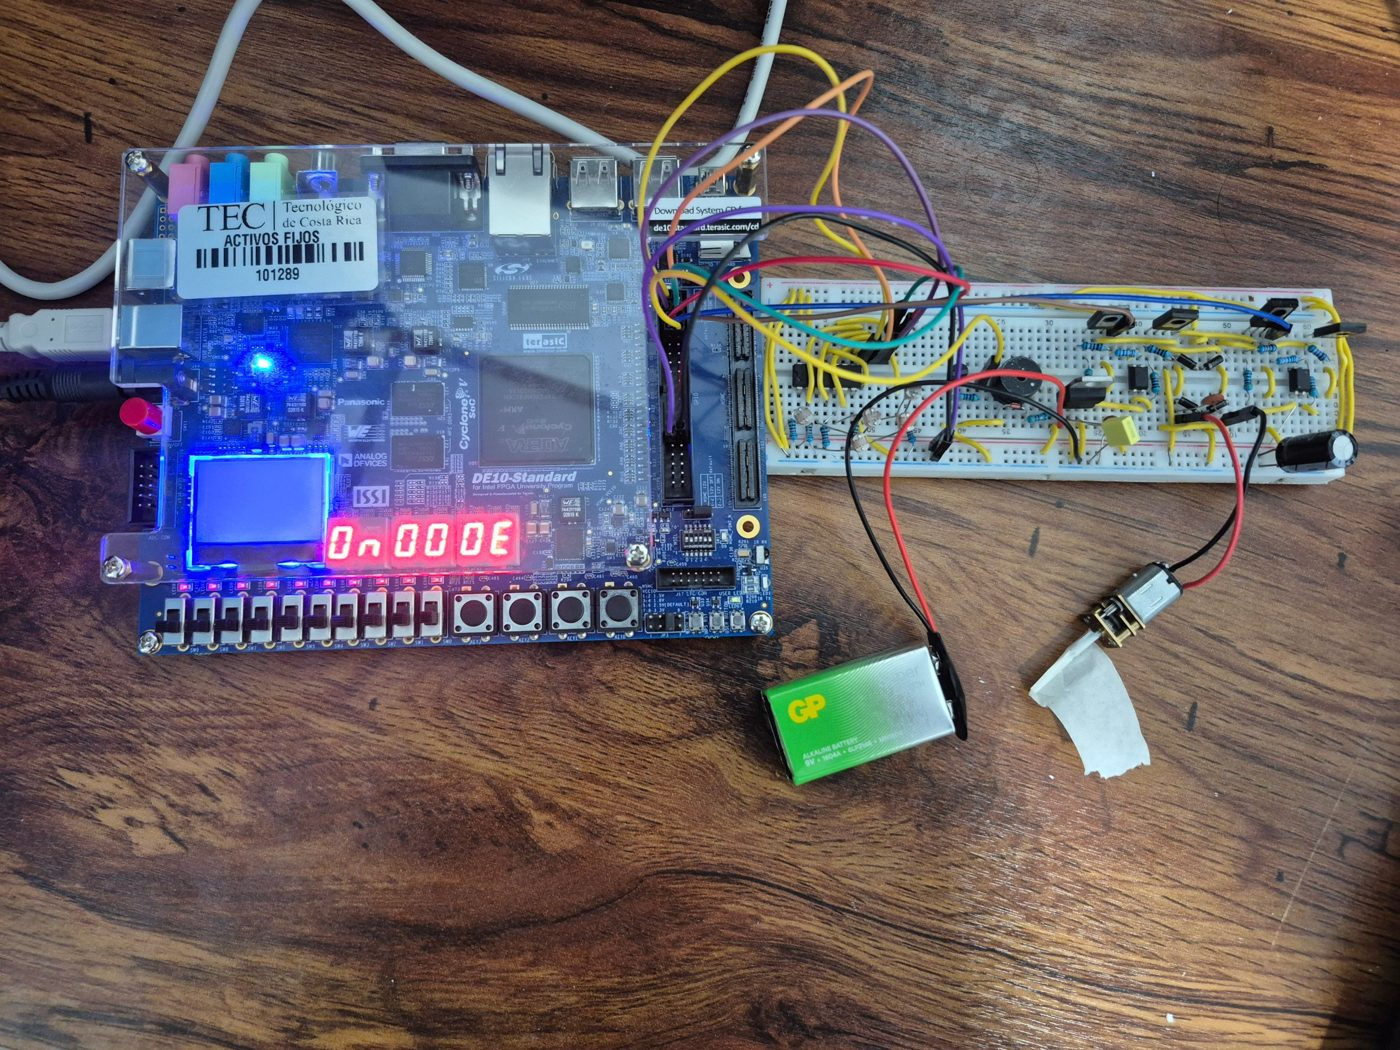
\includegraphics[width=0.85\textwidth]{montaje.jpg}
\caption{Montaje completo. La DE10-Standard está en el
estado inicial (E) y a la derecha se observan la
protoboard con los sensores, el buzzer y la etapa de
potencia, la batería de 9 V y el motorreductor.}
\label{fig:montaje}
\end{figure}

\begin{figure}[!htbp]
\centering
\begin{subfigure}[b]{0.45\textwidth}
    \centering
    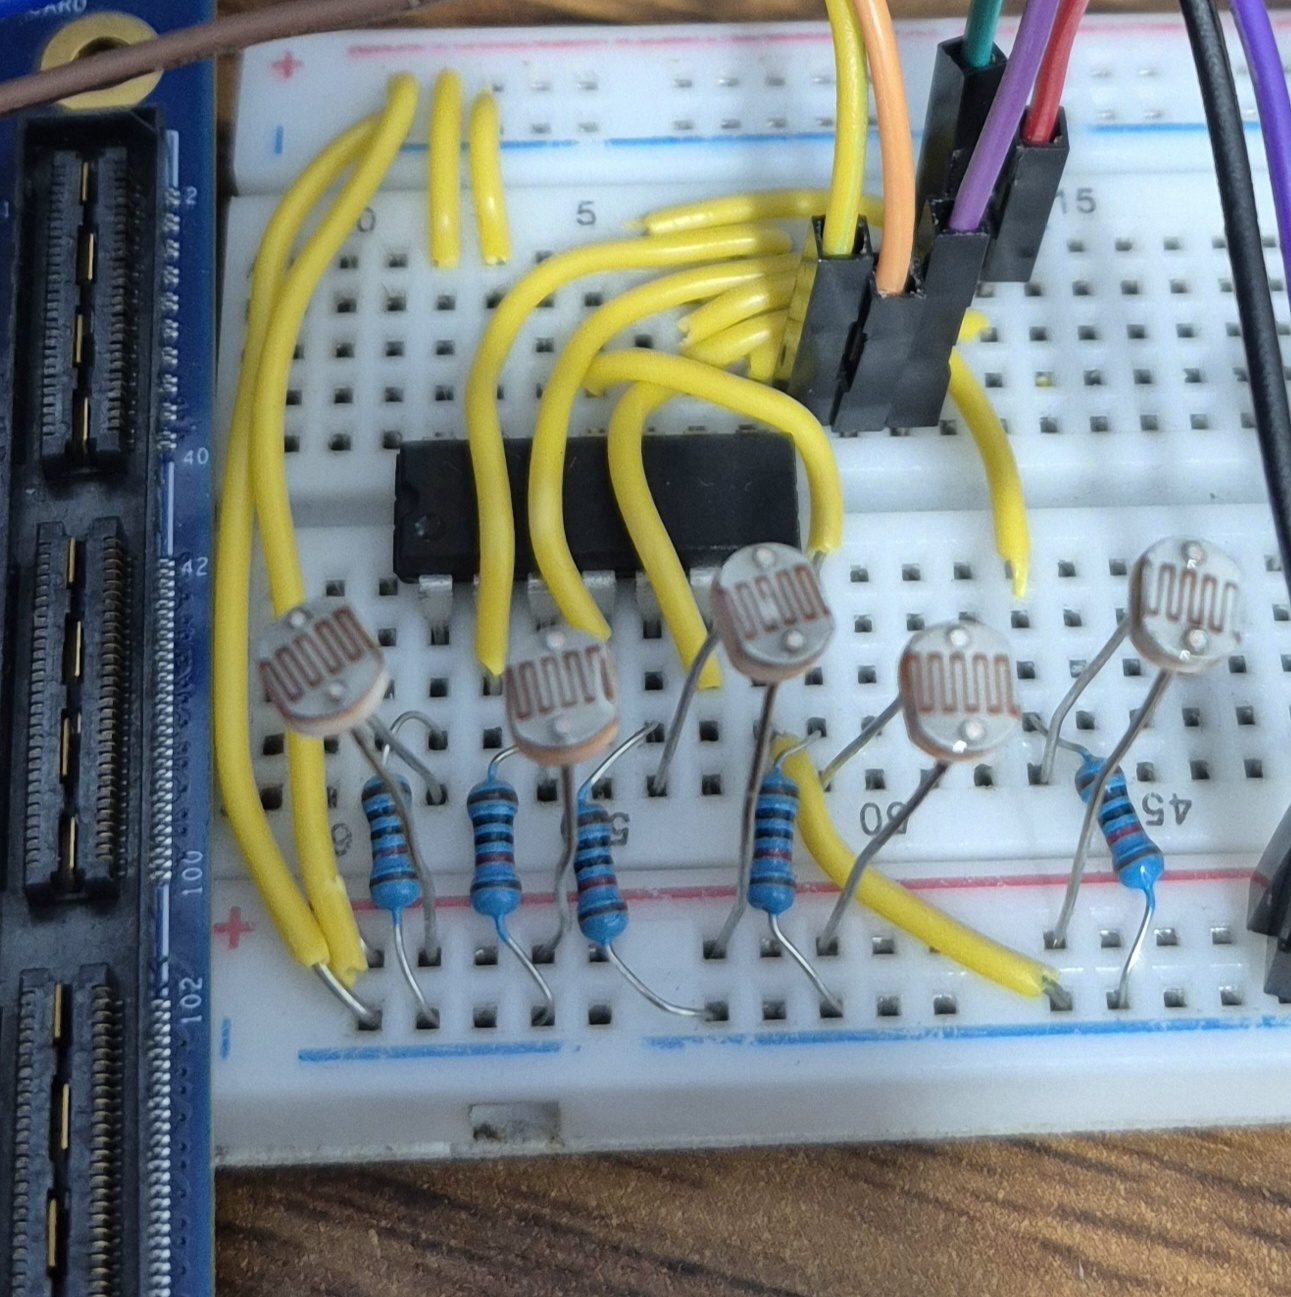
\includegraphics[width=\textwidth]{sensores.jpg}
    \caption{Fotorresistencias, resistencias de
    10 k$\Omega$ y 74HC14.}
\end{subfigure}
\hfill
\begin{subfigure}[b]{0.37\textwidth}
    \centering
    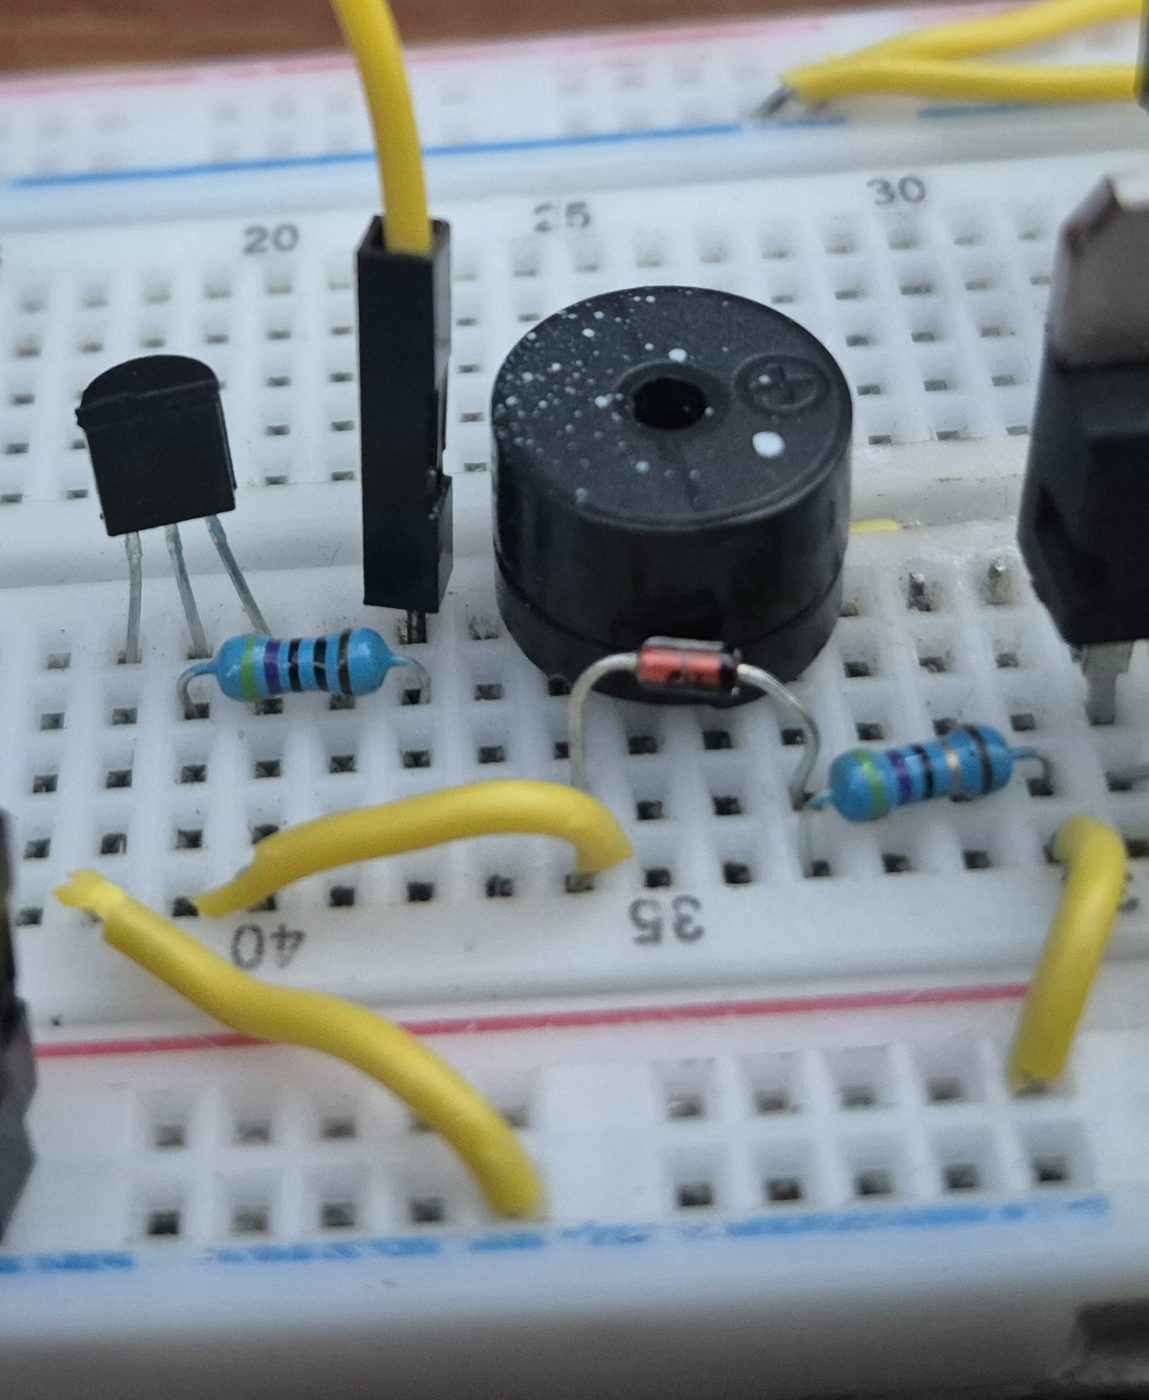
\includegraphics[width=\textwidth]{buzzer.jpg}
    \caption{Buzzer con su transistor 2N3904 y su
    diodo.}
\end{subfigure}

\vspace{0.6em}
\begin{subfigure}[b]{0.85\textwidth}
    \centering
    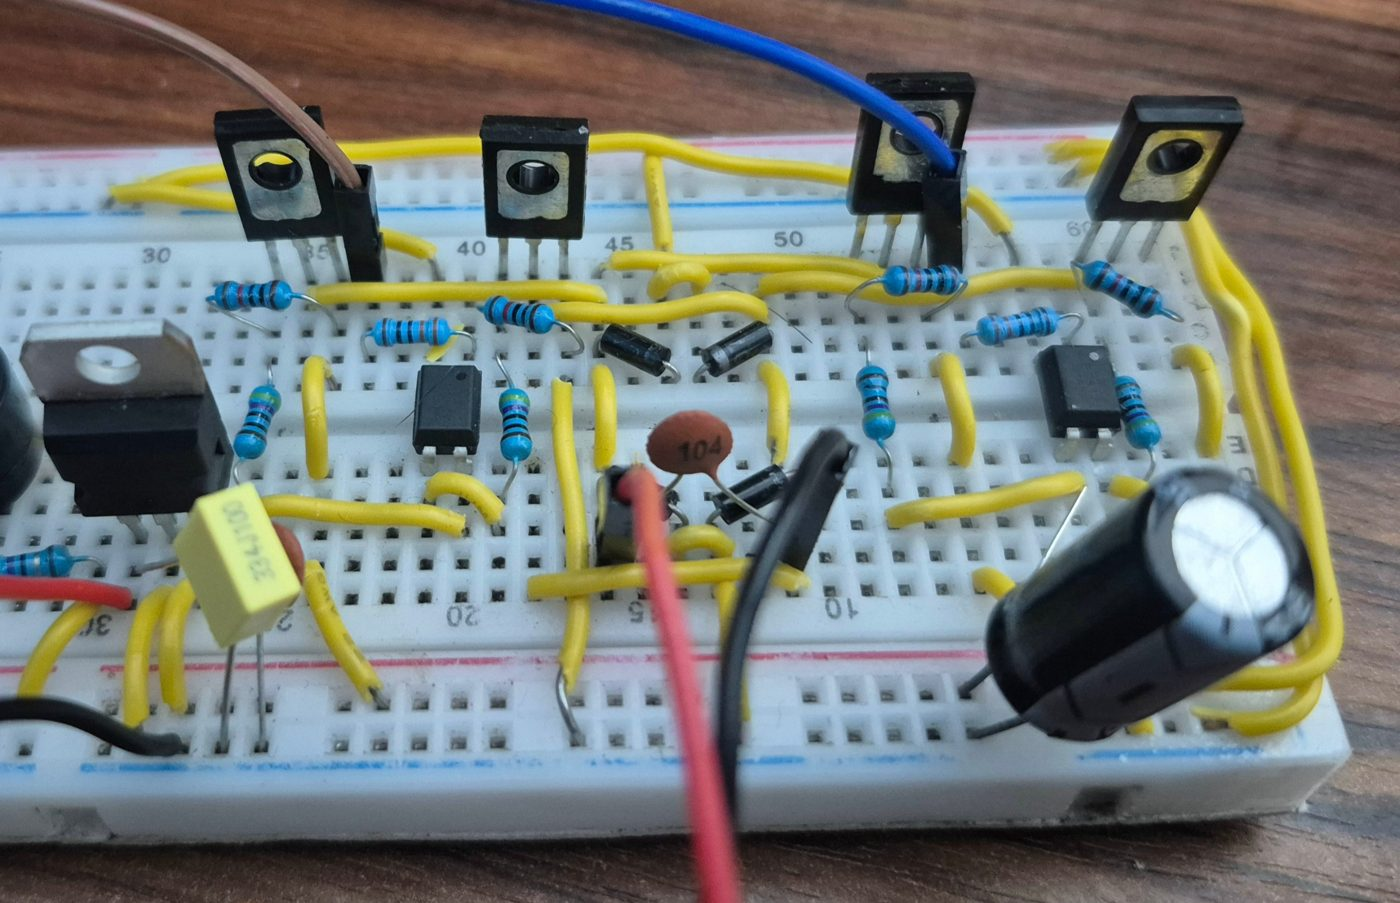
\includegraphics[width=\textwidth]{potencia.jpg}
    \caption{Optoacopladores PC817, puente H y regulador
    de 6 V.}
\end{subfigure}
\caption{Etapas físicas de entrada y salida.}
\label{fig:etapas}
\end{figure}

\begin{figure}[!htbp]
\centering
\begin{subfigure}[t]{0.48\textwidth}
    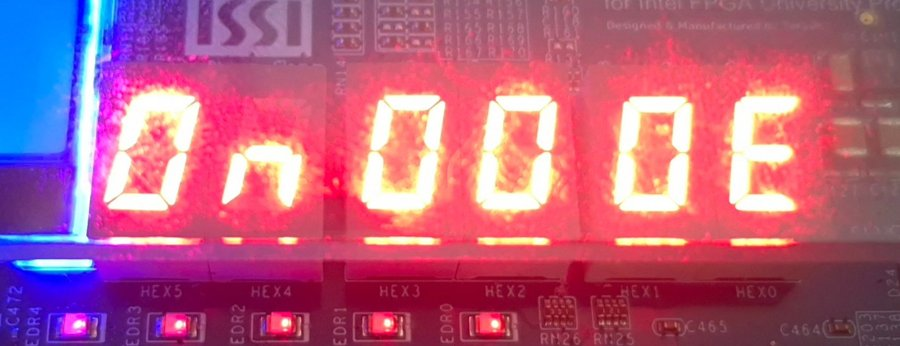
\includegraphics[width=\textwidth]{hex_error.jpg}
    \caption{Encendido sin contraseñas, estado ERROR.}
\end{subfigure}
\hfill
\begin{subfigure}[t]{0.48\textwidth}
    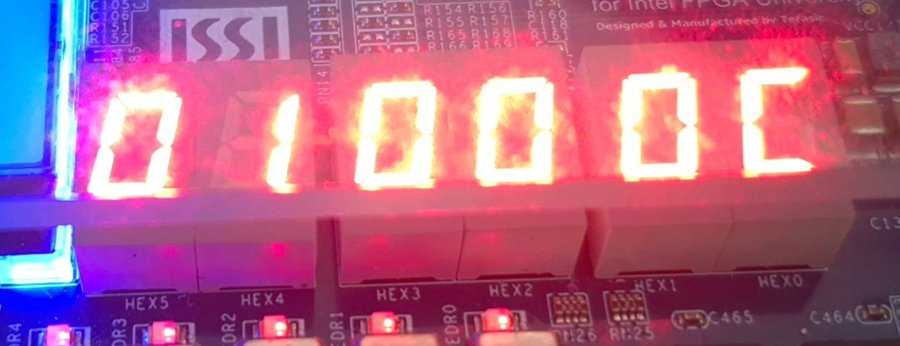
\includegraphics[width=\textwidth]{hex_admin.jpg}
    \caption{Administración en el espacio 1.}
\end{subfigure}

\vspace{0.4em}
\begin{subfigure}[t]{0.48\textwidth}
    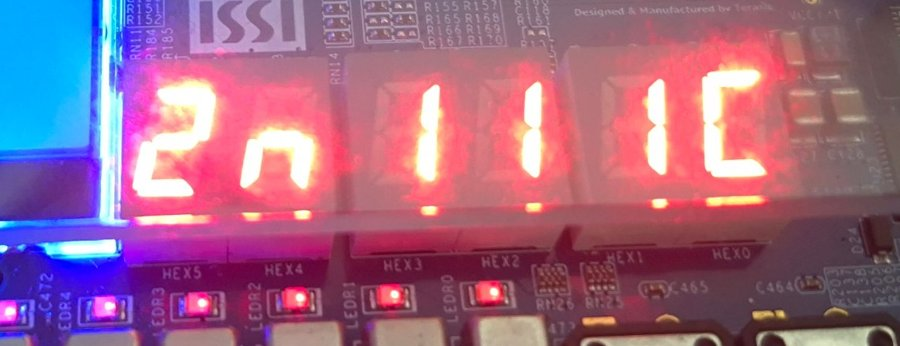
\includegraphics[width=\textwidth]{hex_intento.jpg}
    \caption{Intento 1-1-1 aceptado con velocidad
    $1+1=2$.}
\end{subfigure}
\hfill
\begin{subfigure}[t]{0.48\textwidth}
    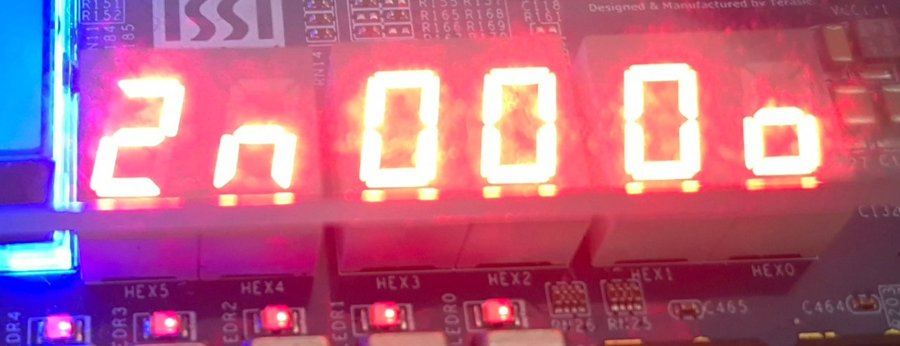
\includegraphics[width=\textwidth]{hex_abriendo.jpg}
    \caption{Apertura (o).}
\end{subfigure}

\vspace{0.4em}
\begin{subfigure}[t]{0.48\textwidth}
    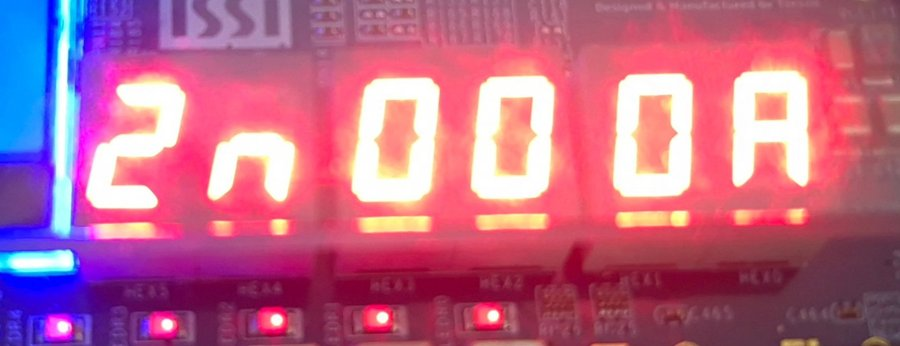
\includegraphics[width=\textwidth]{hex_abierta.jpg}
    \caption{Puerta abierta (A).}
\end{subfigure}
\hfill
\begin{subfigure}[t]{0.48\textwidth}
    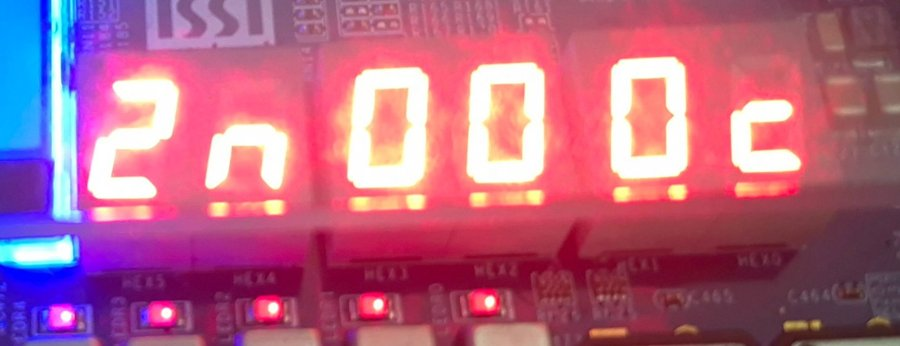
\includegraphics[width=\textwidth]{hex_cerrando.jpg}
    \caption{Cierre (c).}
\end{subfigure}

\vspace{0.4em}
\begin{subfigure}[t]{0.48\textwidth}
    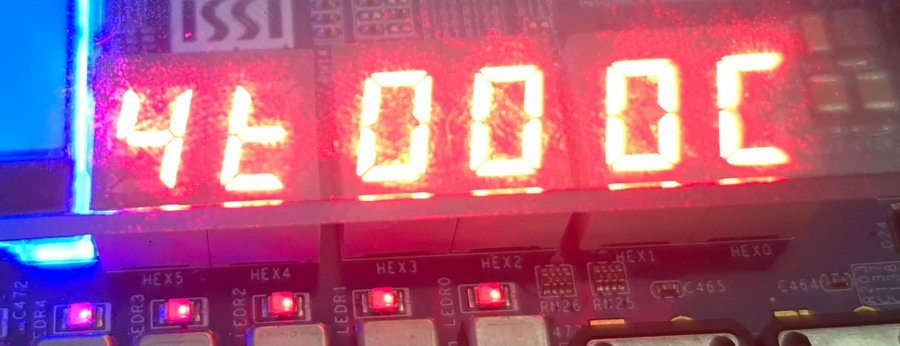
\includegraphics[width=\textwidth]{hex_test.jpg}
    \caption{Prueba (t) a la velocidad fija 4.}
\end{subfigure}
\caption{Estados observados en los displays.}
\label{fig:estados}
\end{figure}

\subsection{Maqueta de la puerta}

La maqueta es una puerta corrediza. Un lazo cerrado de
hilo va del carrete del motor, de 1 cm de diámetro, a una
polea libre en el otro extremo, y el portón se une a uno
de sus tramos con una pestaña pegada al hilo. El portón
se desliza entre dos guías frente a una pared con un
hueco que tapa al cerrar. Se prefirió a una puerta
levadiza porque en el lazo el hilo patina en los topes y
el motor no se fuerza si el recorrido dura más de lo
necesario.

Conectado directo a la fuente, el motor dio unas cinco
vueltas por segundo a 6 V. Con el carrete de 1 cm el hilo
avanza unos 3.77 cm por vuelta, cerca de 18.9 cm/s, de
modo que un recorrido de 20 cm dura alrededor de 1.1 s a
máxima velocidad. Con ese recorrido el portón mide
$20\times12$ cm, la pared $48\times21$ cm con un hueco de
$19\times10$ cm y el piso $48\times12$ cm.

Durante el montaje la polea libre no giraba sobre su eje
y el hilo se arrastraba sobre ella. Más vueltas del hilo
en el carrete aumentaban el agarre, pero concentraban la
fuerza en la polea trabada y terminaron rompiendo el
carrete, por lo que se volvió a un lazo con pocas vueltas
y la tensión mínima para que el hilo no colgara.

Con la maqueta terminada y el PWM a 10 Hz, la puerta abrió
y cerró en los siete niveles, y en cada tope el contacto
detuvo el motor antes de que terminara el tiempo
programado. Los contactos se comprobaron también con el
motor detenido, en cuyo caso no producen ningún cambio.

\textbf{Tiempo de recorrido con el portón.} Se cronometró un
recorrido por nivel, desde que arranca el motor hasta que
el contacto lo detiene, usando el tono del buzzer como
referencia.

\begin{table}[H]
\centering
\begin{tabular}{@{}crrr@{}}
\toprule
$s$ & $T(s)$ programado (s) & Medido (s) & $T(s)/t$\\
\midrule
1 & 28.00 & 4.27 & 6.6\\
2 & 14.00 & 1.93 & 7.3\\
3 & 9.33 & 1.51 & 6.2\\
4 & 7.00 & 1.02 & 6.9\\
5 & 5.60 & 0.67 & 8.4\\
6 & 4.67 & 0.47 & 9.9\\
7 & 4.00 & 0.35 & 11.4\\
\bottomrule
\end{tabular}
\caption{Tiempo de recorrido del portón en la maqueta.}
\label{tab:recorrido}
\end{table}

\subsection{Datos físicos pendientes}

Los recorridos se midieron una sola vez por nivel. Para
calibrar $T(s)$ como respaldo de los contactos se propone
registrar, para cada nivel no nulo, al menos cinco tiempos
de apertura y cinco de cierre, y ajustar los tiempos de
referencia con un margen cercano al 10 \%. Para cada
conjunto de $n$ mediciones se calcularán el tiempo
promedio y la desviación estándar:

\begin{equation}
\overline{t}=\frac{1}{n}\sum_{i=1}^{n}t_i,
\qquad
s_t=\sqrt{\frac{\sum_{i=1}^{n}(t_i-\overline{t})^2}{n-1}}.
\end{equation}

% ============================================================
% 4. ANÁLISIS
% ============================================================

\section{Análisis de los datos obtenidos en el desarrollo
de la investigación}

\subsection{Comportamiento del PWM}

Los conteos observados coinciden con los umbrales
calculados para $D=s/7$. El redondeo introduce un error
inferior a un ciclo de reloj respecto al valor ideal.

En la versión inicial el período de 50\,000 ciclos
correspondía a 1 ms, y en la versión final el período
de 5\,000\,000 ciclos corresponde a 100 ms. En los extremos
la salida permanece constantemente apagada o encendida,
por lo que no se observan transiciones periódicas.

Las mediciones físicas confirman este comportamiento
(tabla~\ref{tab:pwm_fisico}). La tensión promedio crece
0.477 V por nivel, con un ajuste lineal de
$R^2 = 0.999999$ y una ordenada prácticamente nula. Todas
las lecturas quedan alrededor de 1.1 \% por encima de lo
esperado, porque el nivel alto real del pin es 3.338 V y
no 3.300 V. Al normalizar cada lectura con la de $s=7$,
el ciclo de trabajo difiere de $s/7$ en menos de 0.1
puntos porcentuales. Por tanto los siete niveles quedan
repartidos de forma equitativa.

Estos resultados validan la señal que entrega la FPGA.
La relación entre ciclo de trabajo y velocidad real del
motor depende además de la etapa de potencia y del
mecanismo, como se analiza a continuación.

\subsection{Respuesta del motor y elección de la frecuencia}
\label{sec:motor}

Con PWM de 1 kHz el nivel 1 no lograba arrancar el motor,
aunque el pin entregaba la tensión promedio correcta. Con
el motorreductor 150:1 el arranque mejoró, pero las
diferencias entre niveles eran poco visibles. Se atribuye
a dos causas. El optoacoplador y el puente H tardan en
conmutar, por lo que los pulsos cortos llegan deformados
al motor. Además, sin carga el motor sigue girando por
inercia durante el tiempo apagado, lo que reduce la
diferencia aparente entre velocidades.

Al bajar la frecuencia a 200 Hz el motor arrancó en todos
los niveles y las diferencias se hicieron notorias, por lo
que se adoptó 100 Hz para ampliar ese margen.

Con el portón acoplado el motor debe vencer además la
fricción estática del mecanismo, y a 100 Hz el pulso del
nivel 1 dura apenas 1.43 ms. Al bajar a 10 Hz el mismo
nivel entrega pulsos de

\begin{equation}
t_{\mathrm{alto}}(1)=\frac{1}{7}\cdot\frac{1}{10\ \mathrm{Hz}}
\approx 14.3\ \mathrm{ms},
\end{equation}

tiempo suficiente para que el motor reciba la tensión
completa, gane fuerza y arrastre el portón. El costo es
que entre pulsos el motor alcanza a frenarse, lo que se
nota como tirones leves en los niveles 1 y 2. Se aceptó
porque la puerta completa su recorrido en todos los
niveles. La frecuencia final no se midió por falta de
osciloscopio, pero se deriva directamente del contador
de 5\,000\,000 ciclos, cuya exactitud se comprobó en
simulación.

La corriente de 0.03 A a máxima velocidad, sin carga, es
coherente con los cerca de 40 mA que indica el fabricante
a 6 V y queda muy por debajo de lo que soportan el puente
y la batería. No se repitió la medición con el portón
acoplado.

\subsection{Coherencia entre PWM y dirección}

La prueba conjunta registró actividad únicamente en
la línea correspondiente al sentido solicitado.
Las órdenes de detener y de dirección no válida
mantuvieron ambas líneas apagadas, incluso con
velocidad máxima.

En el montaje la apertura y el cierre giraron en sentidos
opuestos y el motor se detuvo al final de cada recorrido,
lo que confirma la separación entre generación de PWM y
selección de dirección. La simulación RTL no demuestra
tiempos muertos durante una inversión, pero la FSM
siempre pasa por un estado sin movimiento entre apertura
y cierre, por lo que el puente nunca recibe ambas órdenes
seguidas.

\subsection{Exactitud del temporizador de recorrido}

Los tiempos cronometrados siguen la relación $T(s)=28/s$
(tabla~\ref{tab:timer}) con una diferencia media de
+0.29 s y una desviación estándar de 0.20 s. La diferencia
no crece con el tiempo programado, como ocurriría con un
error del reloj, sino que se mantiene casi constante. Se
atribuye por tanto al tiempo de reacción al usar el
cronómetro. El temporizador cuenta milisegundos derivados
del reloj de 50 MHz, mucho más preciso que la medición
manual.

Este resultado valida el temporizador, pero no la
duración adecuada del recorrido. En la maqueta el portón
llega a cada tope mucho antes de que termine $T(s)$
(tabla~\ref{tab:recorrido}). El tiempo programado es entre
6 y 11 veces el recorrido real, de modo que en todos los
niveles es el contacto el que corta el movimiento. Si un
contacto falla, el hilo patina en el tope sin forzar el
motor hasta que termina $T(s)$, por lo que los tiempos
actuales sirven como respaldo aunque sean holgados.

El recorrido no baja exactamente como $1/s$. El producto
$s\,t$ ronda 4 s en los niveles bajos y cae a 2.5 s en el
nivel 7, es decir, los niveles altos mueven el portón más
rápido de lo que indica su ciclo de trabajo. Es coherente
con lo observado al ajustar la frecuencia, porque parte de
cada pulso se gasta en vencer la fricción del mecanismo, y
esa pérdida pesa más en los niveles bajos. Además, en los
niveles 5 a 7 los tiempos son menores a un segundo y
quedan cerca del error de unos 0.3 s que mostró el
cronómetro manual en la tabla~\ref{tab:timer}, por lo que
esos valores son solo aproximados.

\subsection{Interpretación de las pruebas del display}

Las 9270 comparaciones comprobaron seis salidas por
cada uno de los 1545 escenarios. Se evaluaron estados,
modos, velocidades, ventanas de captura y reset.

En la FPGA los displays mostraron el carácter esperado en
cada estado (figura~\ref{fig:estados}). Durante el
movimiento HEX0 pasa por o, A y c, y en administración y
prueba conserva la posición recordada de la puerta. En
validación ocurre lo mismo, porque la puerta todavía no
se mueve.

Las pruebas físicas revelaron un problema que la
simulación no mostraba con claridad. La FSM limpia la
ventana al evaluar el intento, de modo que el tercer
dígito casi no alcanzaba a verse. Se agregó en el módulo
superior un registro que mantiene el último intento en
los displays hasta la siguiente captura. También se
corrigió el orden de los dígitos para que el intento se
lea de izquierda a derecha en el mismo orden en que se
ingresó.

Por último, HEX5 pasó a mostrar la velocidad normalizada
entre cero y F con los valores 0, 2, 4, 6, 9, B, D y F,
que corresponden a la ecuación de la sección 2. El banco
del display se actualizó con esa tabla y terminó sin
errores.

\subsection{Integración y consistencia de requisitos}

La inspección permitió identificar diferencias entre
la propuesta y algunos componentes:

\begin{itemize}
    \item La ALU interpreta operaciones entre uno y cinco,
    mientras el tipo de operaciones del paquete conservaba
    una numeración anterior.
    \item El filtro de entradas contenía operadores
    ternarios, aunque el enunciado los prohíbe en el
    circuito sintetizable.
    \item La velocidad del display no estaba normalizada
    a la escala hexadecimal.
    \item El paquete de configuración conservaba constantes
    de la planificación que ningún módulo usaba, y el
    generador de habilitaciones producía un pulso para el
    display que nadie recibía.
    \item Algunos bancos imprimen fallos sin finalizar
    con una condición de error inequívoca para el
    ejecutor automático.
\end{itemize}

Los cuatro primeros puntos se corrigieron. El filtro se
reescribió con máscaras y se comprobó contra la versión
anterior durante 300\,000 ciclos aleatorios sin
diferencias. Se eliminaron las constantes, las señales y
las importaciones sin uso, y se comparó el sistema
completo antes y después de la limpieza con los mismos
estímulos, recorriendo los ocho estados. Las salidas
coincidieron en todos los ciclos salvo en HEX5, que
cambió por la normalización.

Estos hallazgos muestran que la verificación debe
contrastar el diseño con los requisitos, además de
compararlo con su propio banco de pruebas.

\subsection{Representación numérica de los tiempos}

Las expresiones que convierten milisegundos en ciclos
pueden desbordar si la multiplicación intermedia se
realiza con enteros de 32 bits.

Por ejemplo:

\begin{equation}
100 \times 50\,000\,000
=5\,000\,000\,000,
\end{equation}

valor superior al máximo de un entero de 32 bits
con signo. Dividir posteriormente entre mil no recupera
la información perdida por el desbordamiento.

Este problema es relevante porque el módulo superior
entrega al buzzer las duraciones calculadas en el paquete.
Las pruebas aisladas con valores correctos o acelerados
no detectan necesariamente un error en esos parámetros
de integración.

Se corrigió dividiendo primero la frecuencia del reloj
entre mil:

\begin{equation}
\text{ciclos} = \frac{f_{\mathrm{clk}}}{1000}\cdot t_{\mathrm{ms}}
= 50\,000 \times 100 = 5\,000\,000.
\end{equation}

Con este orden el valor intermedio cabe holgadamente en
32 bits y no se pierde precisión, porque 50 MHz es
divisible exactamente entre mil.

\subsection{Límites de la evidencia}

La simulación integral con todos los módulos reales y el
análisis de temporización ya se completaron. Las pruebas
físicas confirmaron además el PWM, el temporizador, los
sensores, el buzzer, los displays y el sentido del motor.

La maqueta comprobó además la apertura y el cierre en
las siete velocidades y el corte del movimiento con los
contactos de final de carrera.

Permanece pendiente la calibración de $T(s)$. Los
recorridos con el portón se midieron una sola vez por
nivel y con cronómetro manual, y los tiempos programados
quedan muy por encima de ellos, de modo que hoy funcionan
solo como respaldo de los contactos. Las mediciones
eléctricas se hicieron también una sola vez por nivel y
con el motor sin carga, y la confiabilidad de los
contactos frente a polvo o desgaste no se evaluó.

% ============================================================
% 5. CONCLUSIONES
% ============================================================

\section{Elaboración de conclusiones a partir de la síntesis
y análisis de los resultados de la investigación}

\begin{enumerate}
    \item La organización en cuatro bloques permite
    distribuir responsabilidades y verificar funciones
    de manera independiente. Las interfaces identificadas
    proporcionan una base concreta para la integración
    del controlador de acceso.

    \item El PWM y el control de motor coinciden con lo
    previsto tanto en simulación como en el montaje. La
    tensión promedio crece linealmente con el nivel de
    velocidad, de modo que los siete niveles quedan
    repartidos de forma equitativa.

    \item La respuesta del motor depende de la frecuencia
    del PWM y no solo del ciclo de trabajo. Bajar de 1 kHz
    a 10 Hz permitió que el motor moviera el portón en
    todos los niveles, lo que muestra que los parámetros
    digitales deben elegirse considerando la etapa de
    potencia y la carga mecánica.

    \item La captura de intentos completos, el
    almacenamiento de velocidad y la separación entre
    reset de encendido y borrado de contraseñas permiten
    expresar explícitamente decisiones temporales del
    sistema. Su funcionamiento conjunto se comprobó en la
    simulación integrada y en la FPGA, donde los displays
    reflejaron cada estado.

    \item La aprobación de un banco de pruebas no
    garantiza cumplimiento del enunciado si la referencia
    utiliza una especificación anterior. La normalización
    del display y los códigos de operación evidencian la
    necesidad de mantener sincronizados requisitos,
    configuración, implementación y pruebas. Ambos casos
    se corrigieron durante la integración, junto con el
    código que había quedado sin uso.

    \item El tamaño de los datos intermedios puede
    modificar el comportamiento del sistema, incluso
    cuando las ecuaciones matemáticas son correctas. El
    desbordamiento se corrigió reordenando la operación, y
    la restricción de reloj permitió confirmar que el
    diseño cumple la temporización a 50 MHz.

    \item La hipótesis de que la modularidad facilita
    detectar problemas recibe apoyo. Cada bloque se
    verificó por separado, la integración funcionó en
    simulación y en la FPGA, y los problemas encontrados
    se localizaron en módulos concretos. Los finales de
    carrera se agregaron solo en el módulo superior, sin
    modificar la FSM, porque llegan por la misma señal que
    el temporizador.

    \item Detectar la llegada a cada tope es más robusto
    que estimarla por tiempo, porque no depende de la carga
    ni de la alimentación. La forma del sensor debe
    escogerse según la fuerza que entrega el mecanismo, y
    su resistencia de pull-up según la resistencia del
    contacto.
\end{enumerate}

% ============================================================
% REFERENCIAS
% Sustituir descripciones generales por las versiones,
% enlaces y fechas reales disponibles en el repositorio.
% No añadir fuentes que no se hayan consultado.
% ============================================================

\begin{thebibliography}{9}

\bibitem{enunciado}
Escuela de Ingeniería en Computadores,
Instituto Tecnológico de Costa Rica.
\textit{Proyecto Grupal 1: Máquinas de estados}.
CE1107, Fundamentos de Arquitectura de Computadores,
2026. Archivo proporcionado:
\texttt{Proyectos\_FAC\_Proyecto\_Grupal1\_v7.pdf}.

\bibitem{propuesta}
Equipo de desarrollo.
\textit{Propuesta del sistema de puerta con contraseña}.
Documentación interna del proyecto,
\texttt{docs/propuesta.md}, versión revisada
el 29 de octubre de 2026.

\bibitem{transcriptA}
Equipo de desarrollo.
\textit{Registros de simulación del Bloque A}.
Archivos de la carpeta
\texttt{docs/simulaciones}, 19 de octubre de 2026.

\bibitem{docsBC}
Equipo de desarrollo.
\textit{Documentación de los bloques de datos y control}.
Carpetas \texttt{docs/BloqueB} y
\texttt{docs/BloqueC}, versión revisada
el 2 de noviembre de 2026.

\end{thebibliography}

\end{document}
